% main.tex
% Fichero principal de transparencias (incluye a todos los demás).

% Compilar a .pdf con LaTeX (pdflatex)
% Es necesario instalar Beamer (paquete latex-beamer en Debian)
%

% Gráficos:
% Los gráficos pueden suministrarse en PNG, JPG, TIF, PDF, MPS
% Los EPS deben convertirse a PDF (usar epstopdf)
%
\documentclass[17pt,aspectratio=169,hyperref=pdfusetitle]{beamer}
\usetheme[orchid]{Hannover}
\beamertemplatenavigationsymbolsempty
\setbeamertemplate{headline}{}
\useoutertheme{infolines}

\usepackage[spanish]{babel}
\usepackage[utf8]{inputenc}
\usepackage{graphics}
%\usepackage{amssymb} % Simbolos matematicos
%\usepackage[pdfusetitle]{hyperref}

\usepackage{chronosys}

%% two slides per page
%\usepackage{pgfpages}
%\pgfpagesuselayout{2 on 1}[a4paper,border shrink=5mm]

\newcommand\YUGE{\fontsize{48}{60}\selectfont}

\newcommand{\secimage}{figs/bookpages}
%\newcommand{\secimage}{figs/keep-calm-lag}
\AtBeginSection[]
{
  {
    \usebackgroundtemplate{\includegraphics[width=\paperwidth,height=\paperheight]{\secimage}}
    \begin{frame}<beamer>

      \begin{center}
        {\YUGE\bf\insertsection}
      \end{center}
    \end{frame}
  }
    \renewcommand{\secimage}{figs/bookpages}
}

%\setbeamersize{text margin left=1em}

\title[Technical lag]{Technical lag for software deployments}
%\subtitle{}
\author[Jesus M. Gonzalez-Barahona]{Jesus M. Gonzalez-Barahona}
\institute[URJC]{Universidad Rey Juan Carlos \\
  @jgbarah ~~~~~ \url{http://github.com/jgbarah/presentations}}

\date[Seminar IMDEA Software ]{Seminar at IMDEA Software \\ Madrid (Spain), October 2nd 2018}

\begin{document}

%\begin{frame}[label=firstframe]
\begin{frame}
  \maketitle
\end{frame}


\begin{frame}

  {\em
    \begin{center}
      %\begin{quote}
      ``If I go there will be trouble \\
      And if I stay it will be double \\
      So come on and let me know''\\
      %\end{quote}
    \end{center}
    \begin{flushright}
      Should I Stay Or Should I Go? \\
      The Clash \\
      \vspace{1cm}
      {\footnotesize
        \url{https://www.youtube.com/watch?v=BN1WwnEDWAM}
      }
    \end{flushright}
  }
\end{frame}


%%%%%%%%%%%%%%%%%%%%%%%%%%%%%%%%%%%%%%%%%%%%%%%%%%%%%%%%%%%%%%%%
%%%%%%%%%%%%%%%%%%%%%%%%%%%%%%%%%%%%%%%%%%%%%%%%%%%%%%%%%%%%%%%%
% lista de temas                                               %
%%%%%%%%%%%%%%%%%%%%%%%%%%%%%%%%%%%%%%%%%%%%%%%%%%%%%%%%%%%%%%%%
%%%%%%%%%%%%%%%%%%%%%%%%%%%%%%%%%%%%%%%%%%%%%%%%%%%%%%%%%%%%%%%%


\definecolor{lightviolet}{HTML}{F4AFF4}
\definecolor{lightorange}{HTML}{FFA17F}
\definecolor{lightgreen}{HTML}{98FB98}
\definecolor{lightred}{HTML}{FF5C5C}
\definecolor{lightblue}{HTML}{89AFCF}
\definecolor{lightbrown}{HTML}{B58868}

%%-----------------------------------------
%%-----------------------------------------
\section{The balance}


%%-----------------------------------------
\begin{frame}[fragile]
  \frametitle{Deployments}

  {\Large
    Any deployment \\
    is the real world instance \\
    of an ``ideal'' target \\
  }
  
\end{frame}

%%-----------------------------------------
\begin{frame}[fragile]
  \frametitle{Deployments: the balance}


    {\Large
    \begin{center}
    ``If it works, don't touch it'' \\
    vs. \\
    ``The quest for the ideal'' \\
    \end{center}
  }
  
\end{frame}

%%-----------------------------------------
\begin{frame}[fragile]
  \frametitle{Deployments: example}

  You want the latest functionality \\
  so you deploy it \\
  but the day after \\
  it is no longer the latest \\

  \begin{flushright}
    Should you update?
  \end{flushright}

\end{frame}

%%-----------------------------------------
\begin{frame}[fragile]
  \frametitle{Living the risky life}

  \begin{center}
  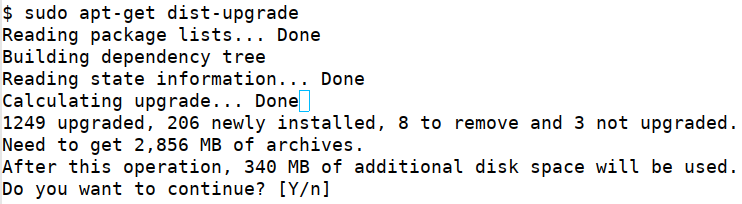
\includegraphics[width=12.5cm]{figs/dist-upgrade}
  \end{center}  

  Upgrading in Debian/testing
  
\end{frame}

%%-----------------------------------------
\begin{frame}[fragile]
  \frametitle{Dependencies}

  You want the latest functionality \\
  so you deploy it \\
  but dependencies may prevent you \\
  from having the latest \\

  \begin{flushright}
    Should dependencies be updated?
  \end{flushright}

\end{frame}

%%-----------------------------------------
\begin{frame}[fragile]
  \frametitle{Living in the past}

\begin{columns}[T]
\begin{column}{.48\textwidth}

  {\footnotesize
\begin{verbatim}
  "dependencies": {
    "coffeescript": "~1.10.0",
    "dateformat": "~1.0.12",
    "eventemitter2": "~0.4.13",
    "exit": "~0.1.1",
    "findup-sync": "~0.3.0",
    ...
  },
\end{verbatim}
  }

\end{column}%
\hfill%
\begin{column}{.40\textwidth}
  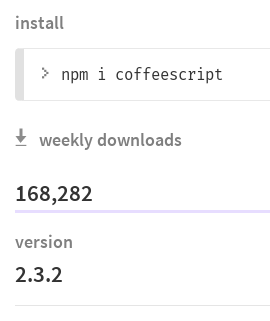
\includegraphics[width=4cm]{figs/coffeescript}
\end{column}%
\end{columns}
  
Oct. 2018: Grunt master / coffescript 
\end{frame}

%%-----------------------------------------
%%-----------------------------------------
\section{Releases}

%%-----------------------------------------
\begin{frame}[fragile]
  \frametitle{Technical lag}

  For a release:

  \vspace{.5cm}
  
  ``difference between the deployed release \\
  and the ideal release'' \\

  \vspace{.5cm}

  \begin{itemize}
  \item What is ``ideal release''?
  \item How we measure difference between releases?
  \end{itemize}
\end{frame}

%%-----------------------------------------
\begin{frame}[fragile]
  \frametitle{Ideal release (examples)}

  Most recent

  Most recent in the stable line

  Less open bugs

  Less unfixed vulnerabilities
  
\end{frame}

%%-----------------------------------------
\begin{frame}[fragile]
  \frametitle{Difference (examples)}

  Difference in release time

  Difference in version number

  Number of commits

  Difference in number of open bugs

  Estimated effort
  
\end{frame}

%%-----------------------------------------
\begin{frame}[fragile]
  %  \frametitle{Formalizing}

  \begin{columns}
    \column{\dimexpr\paperwidth-1cm}
  \begin{itemize}
  \item ideal: $P \times Repos \rightarrow R $ \\
    Given $p \in P$,  $repo \in Repos$, $ideal(p, repo)$ \\

  \item diff: $ R \times R \times Repos \rightarrow L $  \\
    Given $repo \in Repos$ and $r, s \in repo$,  \\
    $diff(r, s, repo)$, if $package(r) = package(s)$

  \item techlag: $R \times Repos \rightarrow L$ \\
    $\forall repo \in Repos, \forall r \in repo$: \\
    $techlag(r, repo) = diff(r, ideal(r, repo), repo)$ \\
  \end{itemize}    

  \end{columns}

\end{frame}

%%-----------------------------------------
\begin{frame}[fragile]
  \frametitle{Example}

\begin{columns}[T]
  \begin{column}{.68\textwidth}
  Package: Pandas \\
  Deployed: 0.22.0 \\
  Ideal: 0.23.4 \\
  \vspace{.5cm}
  Lag (releases): 6 releases \\
  Lag (reltime): 8 months, 4 days \\
\end{column}%
\hfill%
\begin{column}{.30\textwidth}
  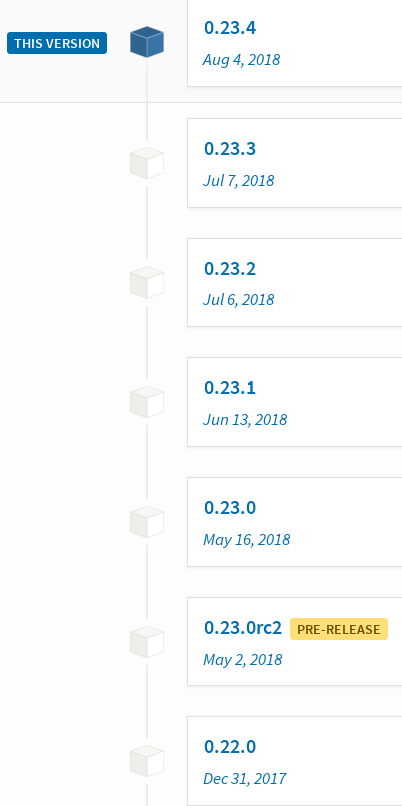
\includegraphics[height=6cm]{figs/pandas}
\end{column}%
\end{columns}
  
\end{frame}


%%-----------------------------------------
\begin{frame}[fragile]
  \frametitle{Example}

\begin{columns}[T]
  \begin{column}{.32\textwidth}
    Debian releases \\
    for git \\
    \vspace{.5cm}
    (source code \& \\
    commits \\
    diffs) \\
\end{column}%
\hfill%
\begin{column}{.70\textwidth}
  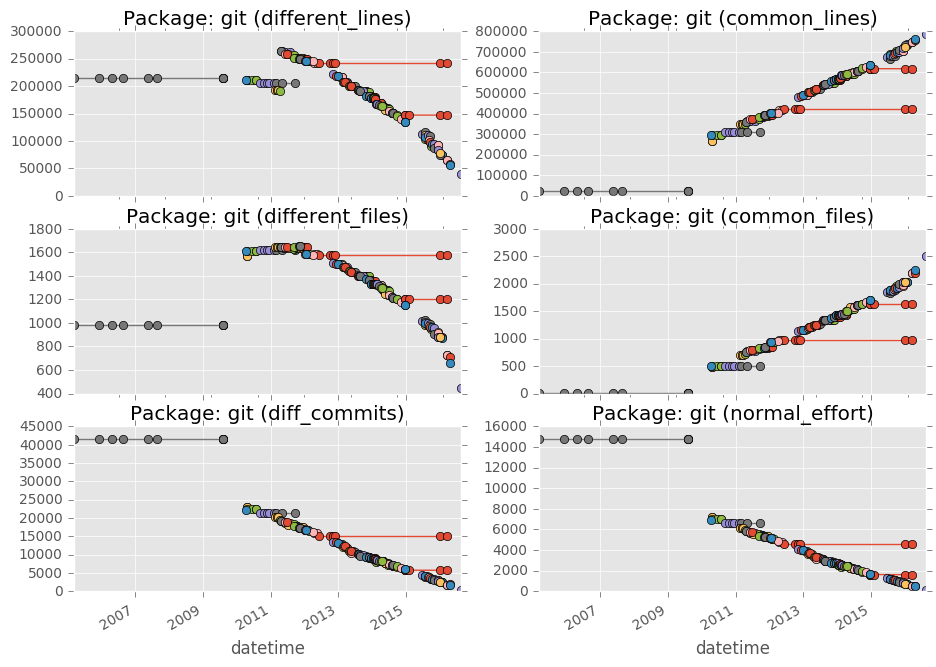
\includegraphics[height=6cm]{figs/git-lags-versions}
\end{column}%
\end{columns}
  
\end{frame}

%%-----------------------------------------
%%-----------------------------------------
\section{Collections}

%%-----------------------------------------
\begin{frame}[fragile]
  \frametitle{Technical lag}

  For a collection of releases:

  \vspace{.5cm}
  
  ``aggregation of the lag \\
  for each release in the collection'' \\

  \vspace{.5cm}

  \begin{itemize}
  \item How do we aggregate?
  \item Examples: maximum, summation, mean
  \end{itemize}
\end{frame}

%%-----------------------------------------
\begin{frame}[fragile]
  %  \frametitle{Formalizing}

  \begin{columns}
    \column{\dimexpr\paperwidth-1.2cm}
  \begin{itemize}
  \item techlag: $ \mathcal P(R) \times Repos \rightarrow L $
  \item   Given $rcoll \in \mathcal P(R), repo \in Repos$, \\
    $techlag_{max}(rcoll, repo) = max_{r\in rcoll}(techlag(r, repo))$ 
  \item   Given $rcoll \in \mathcal P(R), repo \in Repos$, \\
    $techlag_{add}(rcoll, repo) = \sum_{r \in rcoll} techlag(r, repo)$
  \end{itemize}    

  \end{columns}

\end{frame}

%%-----------------------------------------
%%-----------------------------------------
\section{Dependencies (direct)}

%%-----------------------------------------
\begin{frame}[fragile]
  \frametitle{Technical lag}

  For direct dependencies of a release:

  \vspace{.5cm}
  
  ``technical lag \\
  for the collection formed by \\
  direct dependencies of the release'' \\

  \vspace{.5cm}

  \begin{itemize}
  \item Having constraints into account
  \item Selecting as the package manager does
  \end{itemize}
\end{frame}

%%-----------------------------------------
\begin{frame}[fragile]
  %  \frametitle{Formalizing}

  {\small
  \begin{columns}
    \column{\dimexpr\paperwidth-1.5cm}
  \begin{itemize}
  \item $dep: R \rightarrow \mathcal P \left({P}\right)$
  \item $allowed: R \times P \times Repos \rightarrow \mathcal P \left({R}\right)$ \\
    $allowed(r, p, repo) =  rcol$, where $rcol \subset repo$.
  \item $selectver: \mathcal P \left({R}\right) \rightarrow R$ 
  \item $deploy: R \times Repos \rightarrow \mathcal P \left({R}\right)$ \\
    Given $repo \in Repos, r \in repo$, \\
    $deploy(r, repo) =$ \\
    $\{ selectver(allowed(r, p_i, repo)), \forall p_i \in dep(r) \} $
  \item $deplag: R \times Repos \rightarrow L$: $deplag(r, repo) = techlag(deploy(r, repo))$
  \end{itemize}    
  \end{columns}
  }
\end{frame}

%%-----------------------------------------
%%-----------------------------------------
\section{Dependencies (all)}

%%-----------------------------------------
\begin{frame}[fragile]
  \frametitle{Technical lag}

  For all dependencies of a release:

  \vspace{.5cm}
  
  ``technical lag \\
  for the collection formed by \\
  all (transitive) dependencies of the release'' \\

  \vspace{.5cm}

  \begin{itemize}
  \item Having constraints into account
  \item Selecting as the package manager does
  \end{itemize}
\end{frame}

%%-----------------------------------------
\begin{frame}[fragile]
  %  \frametitle{Formalizing}

  {\small
  \begin{columns}
    \column{\dimexpr\paperwidth-1.5cm}
  \begin{itemize}
  \item $deploy^+: R \times Repos \rightarrow \mathcal P \left({R}\right)$
  \item Given $repo \in Repos, r \in repo$, \\
    $deploy^+(r, repo)$ as the minimal fix point such that:\\
    $deploy^+(r, repo) \supseteq deploy(r, repo)$\\
    $deploy^+(r, repo) \supseteq deploy(r', repo) \forall r'\in deploy^+(r, repo)$

  \item $deplag^+: R \times Repos \rightarrow L$: $deplag^+(r, repo) = techlag(deploy^+(r, repo))$
  \end{itemize}    
  \end{columns}
  }
\end{frame}

%%-----------------------------------------
\begin{frame}[fragile]
  \frametitle{Example}

  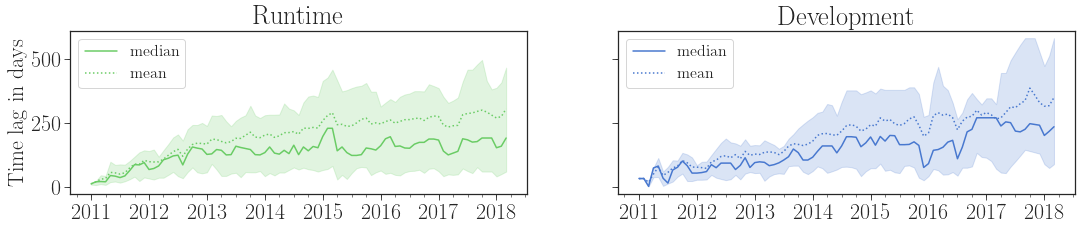
\includegraphics[width=12cm]{figs/npm-time-lag.png}

  npm releases \\
  release time lag, direct dependencies \\

\end{frame}

%%-----------------------------------------
%%-----------------------------------------
\section{Discussion}

%%-----------------------------------------
\begin{frame}[fragile]
  \frametitle{Uses}

  Technical lag of:

  \begin{itemize}
  \item deployed distributions
  \item container images
  \item deployed applications
  \item embedded systems
  \end{itemize}
  
\end{frame}

%%-----------------------------------------
\begin{frame}[fragile]
  \frametitle{Uses}

  Who can control technical lag:

  \begin{itemize}
  \item deployers: ``top level'' releases
  \item developers: direct dependencies
  \item ecosystems: typical dependencies
  \end{itemize}
  
\end{frame}

%%-----------------------------------------
\begin{frame}[fragile]
  \frametitle{Types}

  {\small
  \textbf{Ideal}: latest, most stable, more secure, less buggy... \\

  \textbf{Difference}: \\
  \begin{itemize}
  \item Release metadata: versions, release time...
  \item Source code: diff lines, diff files
  \item SCM: commits, normalized effort
  \item ITS: bugs fixed, vulnerabilities fixed, feature requests closed
  \end{itemize}

  \textbf{Aggregations}: maximum, summation, mean, median \\
  }
\end{frame}

%%-----------------------------------------
%%-----------------------------------------
\section{Summary}

%%-----------------------------------------
\begin{frame}[fragile]

  \includegraphics[width=12cm]{figs/keep-calm-lag}

\end{frame}

%%-----------------------------------------
\begin{frame}[fragile]
%  \frametitle{Summary}

  {\Large
    Difference between real and ideal \\
    \vspace{.5cm}
    What am I missing if I upgrade? \\
    \vspace{.5cm}
    Dependencies impact on lag \\
  }
\end{frame}

%%-----------------------------------------
\begin{frame}[fragile]
  \frametitle{More info...}

{\small
  Ahmed Zerouali, Eleni Constantinou, Tom Mens, Gregorio Robles, Jesús M. González-Barahona: \\
  ``An Empirical Analysis of Technical Lag in npm Package Dependencies'' \\
  ICSR 2018: 95-110 \\

  \vspace{.5cm}
  
  Jesús M. González-Barahona, Paul Sherwood, Gregorio Robles, Daniel Izquierdo-Cortazar: \\
  ``Technical Lag in Software Compilations: Measuring How Outdated a Software Deployment Is'' \\
  OSS 2017: 182-192 \\
}  
\end{frame}


\frame{
~
\vspace{1cm}

\begin{flushright}


\includegraphics[width=2.2cm]{figs/by-sa}
 \\

\begin{footnotesize}
\copyright 2018 Jesus M. Gonzalez-Barahona. \\

\vspace{.4cm}

Some rights reserverd. This document is distributed under the terms of the Creative Commons License ``Attribution-ShareAlike 4.0'',
available in \\
{\scriptsize \url{http://creativecommons.org/licenses/by-sa/4.0/}} \\

\vspace{.4cm}

This document (including source) is available from
\url{https://github.com/jgbarah/presentaciones}

\end{footnotesize}
\end{flushright}

}
%%

%\againframe{firstframe}

\end{document}
